\section{Methods}
\label{sec:methods}


 %%%%%%%%%%%%%%%%%%%%%%%%%%%%%%%%%%%%%%%%%%%%%%%%%%%%%%%%%%%%%%%%%%
 %%%%%%%%%%%%%%%%%%%%%%%%%%%%%%%%%%%%%%%%%%%%%%%%%%%%%%%%%%%%%%%%%%

\subsection{Source Iteration}
Source iteration is Picard iteration for the fixed point problem. We begin with an initial guess $\phi_0$ and solve Equation \ref{eq:transport} for $\psi_1$. Given that:

\begin{equation}
	\label{eq:phi}
	\phi_n = \int_{-1}^{1}\psi_n d\mu .
\end{equation}

That is, given $\phi_n$ compute $\psi_{n+1}$, then compute $\phi_{n+1}$ given Equation \ref{eq:phi} until convergence where $\phi_{n+1} = \phi_{n}$. Given this iterative scheme, Equation \ref{eq:transport} and Equation \ref{eq:phi} combine to become:

\begin{equation}\label{equation:SI}
    \mu\frac{\partial\psi_{n+1}}{\partial x}(x,\mu)+ \Sigma_t(x)\psi_{n+1}(x,\mu) = \frac{1}{2} \left[ \Sigma_s(x)\phi_{n}(x) + q(x)\right].
\end{equation}

Given an angular discretization, this becomes a linear system of equations which, can be represented in operator notation where:
\[
	\phi = \cals(\phi, q, \psi_l, \psi_r)
\]
and
\[
	\calk(\phi) = \cals(\phi, 0, 0, 0) \mbox{ and }
	f = \cals(0, q, \psi_l, \psi_r).
\]
Where Source Iteration is represented as
\[
	\phi_{n+1} = \calk(\phi_n) + f,
\]
to get
\[
	A \phi \equiv (I - \calk) \phi = f
\]
which we can send to a linear solver. It is important to note that the methods employed ensure that we never form the matrix $A$.  Instead, the Monte Carlo simulation will compute the action of matrix $A$ on $\phi$.

 %%%%%%%%%%%%%%%%%%%%%%%%%%%%%%%%%%%%%%%%%%%%%%%%%%%%%%%%%%%%%%%%%%
 %%%%%%%%%%%%%%%%%%%%%%%%%%%%%%%%%%%%%%%%%%%%%%%%%%%%%%%%%%%%%%%%%%

%\subsection{The Matrix-Vector Product}

 
 %%%%%%%%%%%%%%%%%%%%%%%%%%%%%%%%%%%%%%%%%%%%%%%%%%%%%%%%%%%%%%%%%%
 %%%%%%%%%%%%%%%%%%%%%%%%%%%%%%%%%%%%%%%%%%%%%%%%%%%%%%%%%%%%%%%%%%

\subsection{Krylov Subspace Methods}

An order-$r$ Krylov subspace is defined with notation from the previous section as:
\begin{equation}
K_r = \textrm{span}(\phi, A\phi, A^{2}\phi, ..., A^{r-1}\phi).
\end{equation}

For each experiment, two Krylov methods \cite{ctk:roots}, GMRES \cite{gmres} and Bi-CGSTAB \cite{bicgstab}, were used. The Generalized Minimum RESidual (GMRES) is one of the most common Krylov methods. When solving $A\vec{\phi}=\vec{f}$, GMRES minimized $||f-A\phi||_2$ over the $k^{th}$ Krylov subspace. For every iteration, the GMRES stores an additional Krylov vector. For problems that require many iterations this may lead to memory constraints. Bi-CGSTAB is a low-storage Krylov method that is memory bounded throughout the algorithm. However, the memory savings come from information that is thrown out with each iteration and therefore Bi-CSTAB will generally require more iterations to converge than GMRES. Nonetheless, as we will in section \ref{sec:results}, both Krylov methods will require far fewer iterations than the standard SI. 


 %%%%%%%%%%%%%%%%%%%%%%%%%%%%%%%%%%%%%%%%%%%%%%%%%%%%%%%%%%%%%%%%%%
 %%%%%%%%%%%%%%%%%%%%%%%%%%%%%%%%%%%%%%%%%%%%%%%%%%%%%%%%%%%%%%%%%%

\subsection{Monte Carlo Sweep}

Monte Carlo methods for neutron transport seek to simulate the behavior of a statistically significant number of particles from \textit{birth} to \textit{death} to gain an approximate behavior of the system. For our 1-dimensional simulations, each particle begins with an initial position ($x_i$), direction ($\mu_i$), and statistical weight ($w_i$). In an analog simulation, the particle would then be tracked from collision to collision, tallying quantities of interest in a defined spatial mesh. Each time the particle undergoes a collision, a new direction ($\mu$) would be sampled and the next distance to collision would be calculated. This process would repeat until the particle is either absorbed or exits the volume. However, the invoked iterative methods allow the simulation to be modeled as a purely absorbing system. MC simulation in a purely absorbing system can be enhanced by employing the continuous weight absorption technique, which continuously reduces the statistical weight of each particle per length traveled ($s$):
\begin{equation}
    \label{equation:7}
    w_{1} = w_{0}e^{-\Sigma_{a}s}.
\end{equation}
Consequently, after emission the particle is traced straight out of the volume reducing the statistical weight according to the distance traveled across each spatial cell.

The track-length tally estimator is used to calculate the spatially-averaged scalar flux in the defined mesh. Because the weight is continuously reduced with each step, the tally scoring becomes:
\begin{equation}
    \label{equation:8}
    \frac{1}{V}\int_{0}^{s}w_{o}e^{\Sigma_{a}s\prime}ds = \frac{1}{V}\left(\frac{1-w_{o}e^{-\Sigma_{a}s}}{\Sigma_{a}}\right).
\end{equation}
%\subsubsection{Multigroup Equations}

Neutron cross sections vary greatly with energy and contain large resonance regions, making them computationally expensive to model with high fidelity. The multigroup method is a common approach used to model energy-dependent cross sections in Monte Carlo. The multigroup method splits the energy range into $G$ finite regions each with a representative cross section. In general geometry, the multigroup equations for $G$ groups are:
\begin{equation}\label{eq:MG}
\mu  \frac{\partial \psi_g}{\partial x} (x,\mu) + \Sigma_{t,g}(x) \psi_g(x,\mu) =
\frac{1}{2} \sum_{g'=1}^G \Sigma_{s,g'\rightarrow g}(x) \int_{-1}^1 \psi_{g'}(x, \mu') \dmup + \frac{q_g(x)}{2} \quad g=1,\dots,G.
\end{equation}The boundary conditions become:
\[
\psi_g(0, \mu) = \psi_{l,g}(\mu), \mu > 0; \psi_g(\tau, \mu) = \psi_{r,g}(\mu),
\mu < 0.
\]

In matrix form, these equations are
\begin{equation}\label{eq:MGmat}
\mu  \frac{\partial \vec{\psi}}{\partial x} (x,\mu) + \underline{\Sigma}_{t}(x) \vec{\psi}(x,\mu) =
\frac{1}{2}  \underline{\Sigma}_{s}(x) \int_{-1}^1 \vec{\psi}(x, \mu') \dmup + \frac{\vec{q}(x)}{2},
\end{equation}
where
\begin{equation}\label{eq:vecs}
\vec{\psi} = (\psi_1, \psi_2, \dots, \psi_G)^\mathrm{T}, \qquad \vec{q} = (q_1, q_2, \dots, q_G)^\mathrm{T}, 
\end{equation}
\begin{equation}\label{eq:MatricesT}
 \underline{\Sigma}_{t}(x)  = \begin{pmatrix} \Sigma_{t,1}(x) & 0 & \dots\\
 0 & \Sigma_{t,2}(x) & 0 \dots \\
 \vdots & & \ddots\\ 
 0 & \dots & 0 & \Sigma_{t,G}(x) 
 \end{pmatrix}, 
\end{equation}
and
\begin{equation}\label{eq:MatricesS}
 \underline{\Sigma}_{s}(x)  = \begin{pmatrix} \Sigma_{s,1\rightarrow 1}(x) & \Sigma_{s,2\rightarrow 1}(x)  & \dots & \Sigma_{s,G\rightarrow 1}(x) \\
 \Sigma_{s,2\rightarrow 1}(x) & \Sigma_{s,2\rightarrow 1}(x)  & \dots & \Sigma_{s,G\rightarrow 2}(x) \\
 \vdots & \vdots & & \vdots\\
 \Sigma_{s,G\rightarrow 1}(x) & \Sigma_{s,G\rightarrow 1}(x)  & \dots & \Sigma_{s,G\rightarrow G}(x) \\
 \end{pmatrix}.
\end{equation}

\subsubsection{Quasi-Monte Carlo}

Quais-Monte Carlo uses quasi-random low-discrepancy sequences in place of pseudo-random number generators in MC simulations. Low-discrepancy sequences use deterministic algorithms to sample the phase space in \textit{self-avoiding}  manner thereby approaching a more uniform distribution and approximating the expectation more efficiently. This results in a theoretical convergence rate of $O(N^{-1})$ compared to the $O(N^{-0.5})$ from pseudo-randomly placed points \cite{Palluotto2019}.  Because the low-discrepancy sequences sample the phases-space in a deterministic manner they introduce a dependence, albeit a weak one, on the dimensionality of the problem \cite{Hickernell2002}. Commonly used low-discrepancy sequences include the Halton Sequence and Sobol Sequence \cite{Niederreiter1992}. For low-dimensional problems, the Halton sequence has been shown to provide the best results. However, for higher-dimensional problems the Sobol Sequence is most commonly used.

QMC is commonly used in Finance to evaluate high-dimensional integrals \cite{Dagpunar2007} and there has also been recent work in using QMC in radiative heat transfer applications \cite{MOROKOFF1993, Palluotto2019}. However, QMC has largely been ignored by the particle transport community \cite{Spanier1995}. This is because the deterministic nature of the low discrepancy sequence breaks the Markovian assumption needed for the particle \textit{random walk}. Therefore QMC must be implemented in specific applications which are not Markovian processes, such as the initial starting position of each particle, or steps must be take to ensure the Markovian assumption is held. Presently, there have been two separate strategies for implementing QMC in particle transport while maintaining the Markovian assumption. The first is known generally as randomized-QMC or (RQMC) which includes a host of strategies that attempt to reorder the sequence so each point is individually uniformly distributed within the space but the collective still retain their low-discrepency. \cite{Fox1999, Spanier1995, Farmer2020, MOROKOFF1993, Konzen2019}. The second, makes use of the previously discussed  deterministic and iterative methods in which the problem can be modeled in the Monte Carlo simulation as a purely absorbing problem and the scattering term is iterated upon using one of the previously discussed methods removing the need for a \textit{random walk} process \cite{Pasmann2021}.

\begin{figure}[h]
\centerline{
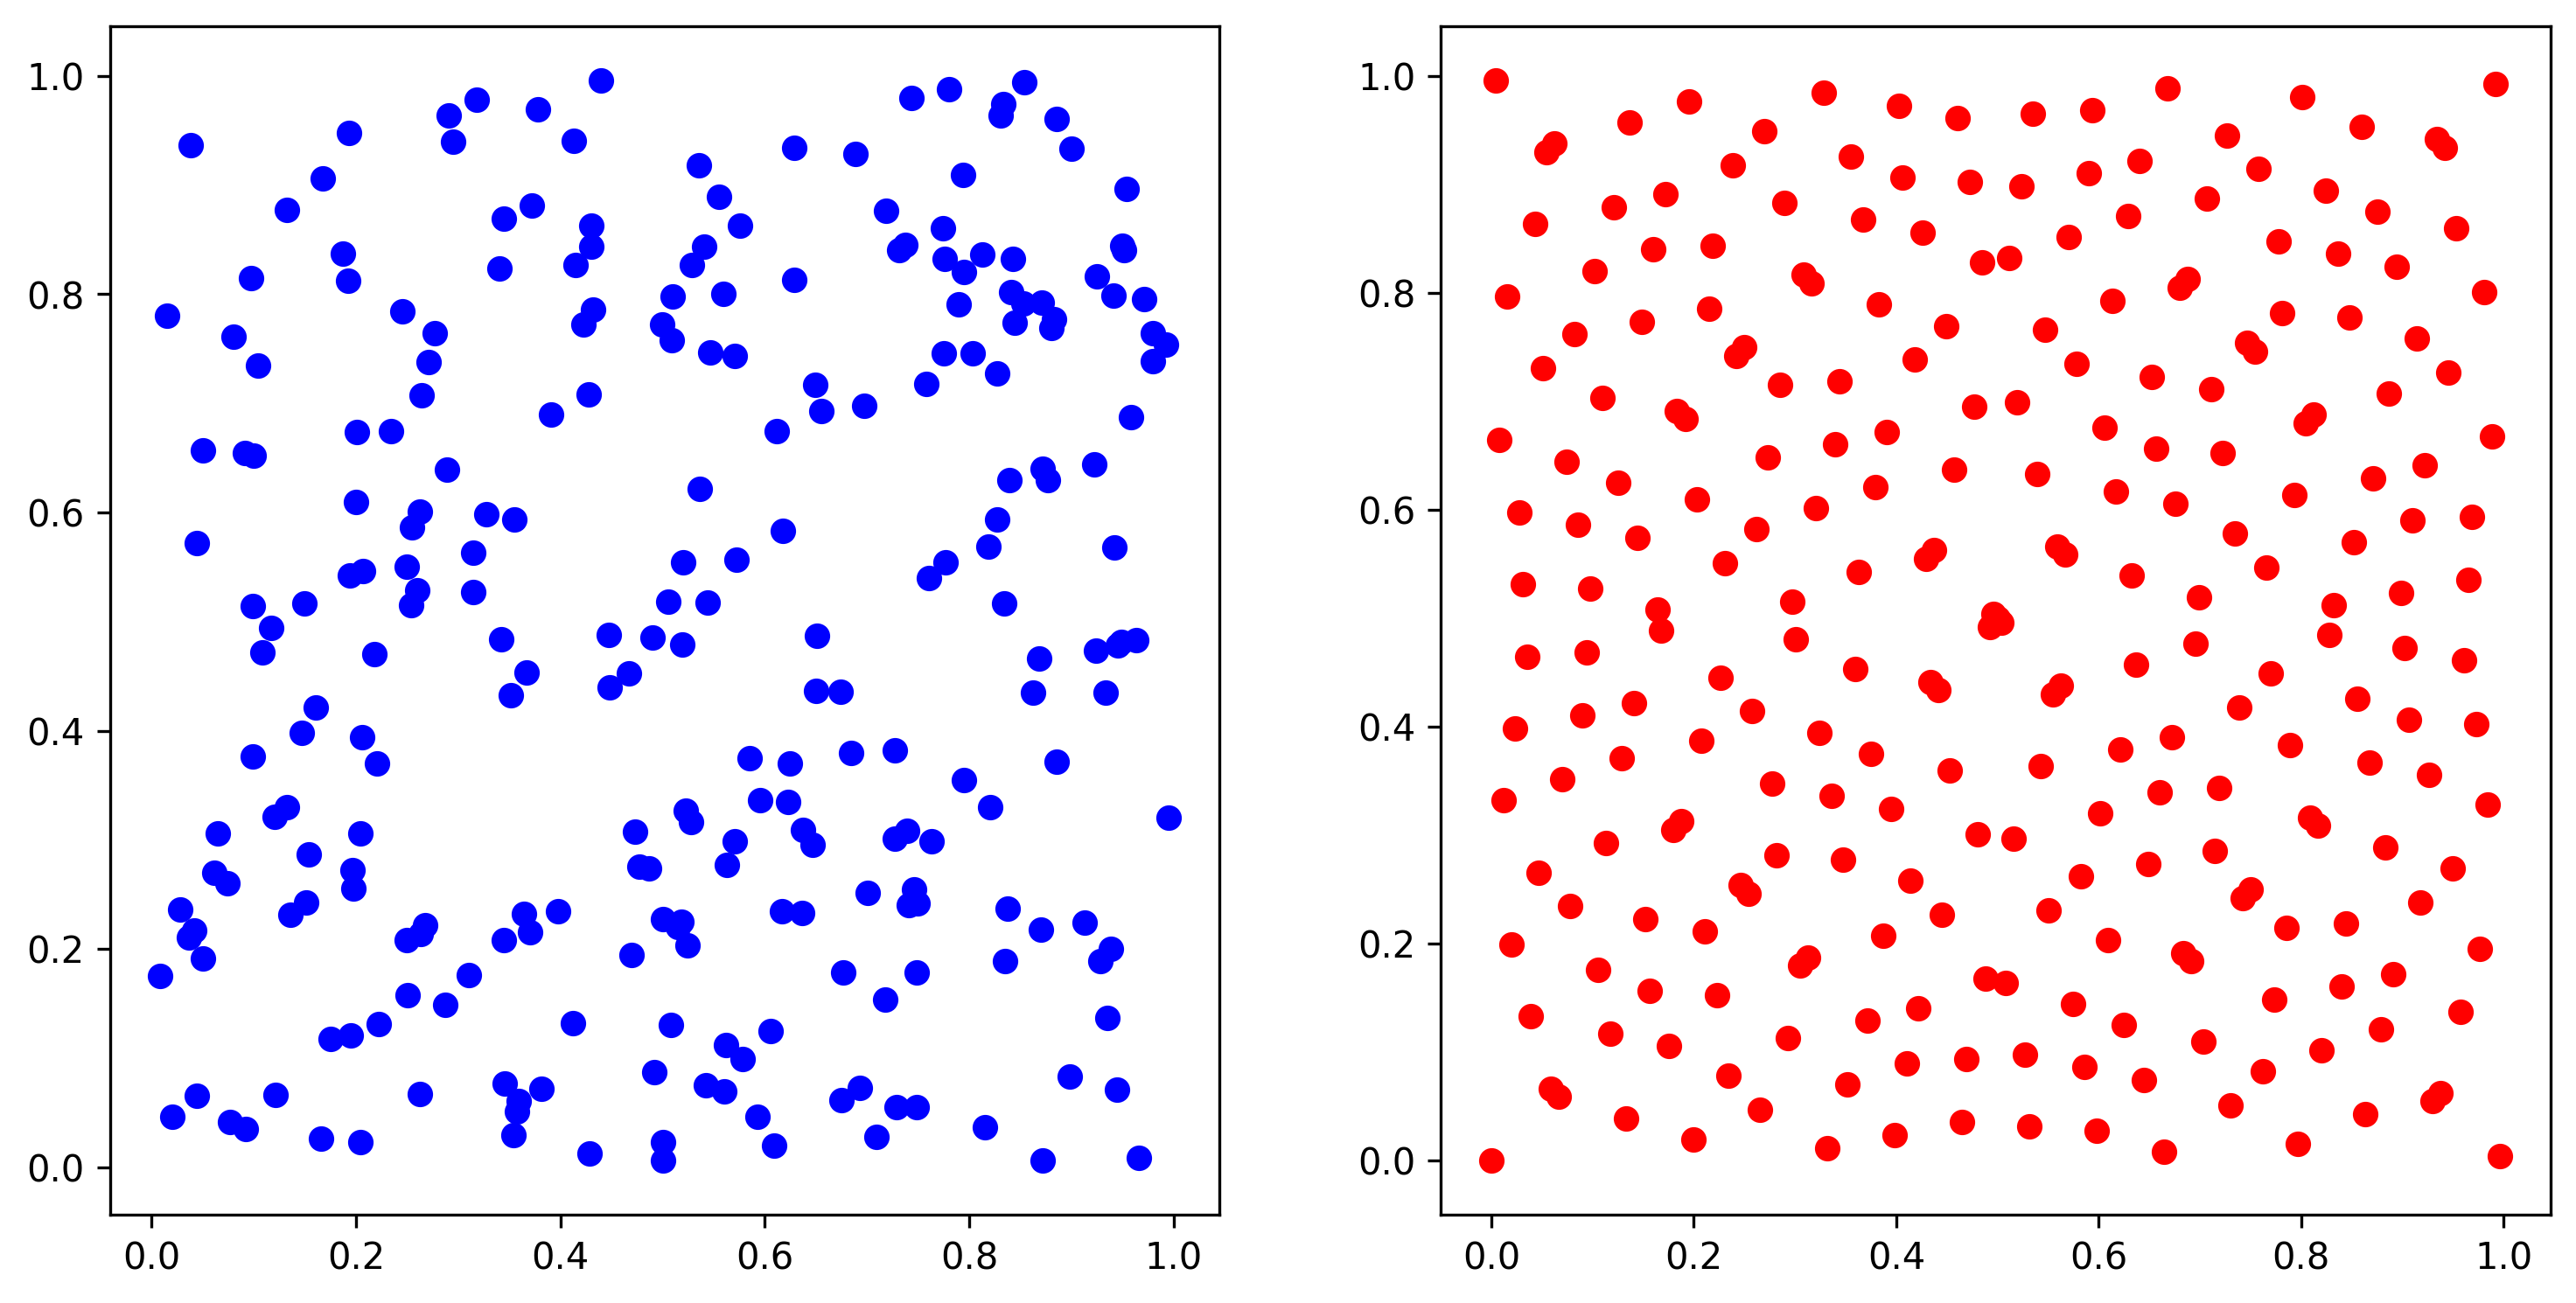
\includegraphics[width=3.5in]{FIGURES/sobol.png}
}
\caption{\label{fig:sobol} 256 points generated in a unit square with pseudo random points (left) and the Sobol sequence (right).}
\end{figure}

